\subsubsection{Elecci�n}
\begin{frame}
\frametitle{}

\begin{figure}
\begin{tikzpicture}[node distance=0.5cm, auto,>=latex', thick]
\scriptsize
    % We need to set at bounding box first. Otherwise the diagram
    % will change position for each frame.
    \path[use as bounding box] (-1.5,0) rectangle (12,-2);

    % TT methodology     
    \node [phase]                        (monitoreo)     {Vigilancia};
    \node [phase2,below of=monitoreo]    (choice)        {Elecci�n};
    \node [phase, below of=choice]       (acquisition)   {Adquisici�n};
    \node [phase, below of=acquisition]  (adaptation)    {Adaptaci�n};
    \node [phase, below of=adaptation]   (absortion)     {Absorci�n};
    \node [phase, below of=absortion]    (aplication)    {Aplicaci�n};
    \node [phase, below of=aplication]   (difusion)      {Difusi�n};

    %%%%%%%%%%%%%%%%%%%%%%%%%%%%%%%%%%%%%%%%%%%%&
    %            Elecci�n
    %%%%%%%%%%%%%%%%%%%%%%%%%%%%%%%%%%%%%%%%%%%%&
    \onslide<1> \node [ph_explain, right=.5cm of adaptation.east] (exp_choice)        
    { \begin{center} \textbf{Elecci�n} \end{center}
      \begin{itemize}
       \item Evaluaci�n del estado de la plataforma tecnol�gica existente para identificar facilidades y necesidades.
       \item Encontrar una tecnolog�a que pueda ser implementada con el estado actual de la plataforma tecnol�gica.
       \item Identificar los niveles de complejidad, para determinar una alternativa que pueda implementarse y de resultados a mediano y corto plazo con no muy altas inversiones de capital.
      \end{itemize}
    };
    

    \onslide<2> \node [ph_explain, right=.5cm of adaptation.east] (exp_choice)        
    { \begin{center} \textbf{Elecci�n} \end{center}
      \begin{center} 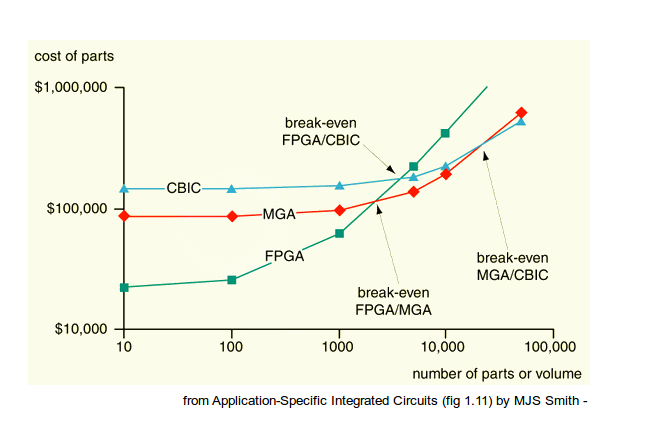
\includegraphics[scale=.55]{../images/GA_vs_ASIC_vs_FPGA.png} \end{center}
      \caption{Comparaci�n de costos entre FPGAs, arreglos de compuertas y ASICs basado en celdas est�ndar, Fuente: Application-Specific Integrated Circuits, MJS Smith} 
    };


\end{tikzpicture}
\end{figure}

\end{frame}